\section{*应用：局部同调群与流形}
\sourcepage{227--228}
本节定义空间在一点处的局部同调群，并用它证明关于流形的若干非平凡事实。全节假设 $X$ 是 Hausdorff 空间。本节将作为第八章的预备知识，第 4.12 节的一个例子也将用到它。

\entry{定义}{4.8.1}空间 $X$ 在点 $x\in X$ 处的\textbf{局部同调群}（local homology groups）是奇异同调群 $H_p(X,X\setminus\{x\})$。

\entry{引理}{4.8.2}若 $A\subset X$ 包含 $x$ 的一个邻域，则
\[
H_p(X,X\setminus\{x\})\cong H_p(A,A\setminus\{x\}).
\]
因此，若 $x\in X$、$y\in Y$ 分别有邻域 $U,V$，使 $(U,x)$ 与 $(V,y)$ 同胚，则两点处的局部同调群同构。这解释了“局部”一词。

\textbf{证明：}令 $U=X\setminus A$。因 $A$ 包含 $x$ 的邻域，$\overline U\subset X\setminus\{x\}=\Int(X\setminus\{x\})$。切除定理给出
\[
H_p(X,X\setminus\{x\})\cong H_p(X\setminus U,(X\setminus\{x\})\setminus U)=H_p(A,A\setminus\{x\}).
\]
\hfill$\square$

\entry{例}{4.8.3}若 $x\in\R^m$，则 $H_i(\R^m,\R^m\setminus\{x\})$ 在 $i=m$ 时为无限循环群，其余为零。取以 $x$ 为中心的正半径闭球 $B$。由上一个引理，
\[
H_i(\R^m,\R^m\setminus\{x\})\cong H_i(B,B\setminus\{x\})\cong H_i(B^m,B^m\setminus\{0\}).
\]
球面 $S^{m-1}$ 是 $B^m\setminus\{0\}$ 的形变收缩核（图 4.8.1，形变公式见定理 2.7.11 的证明），故最后一个群同构于 $H_i(B^m,S^{m-1})$。由定理 4.4.11 即得结论。

\entry{例}{4.8.4}记欧氏半空间
\[
\mathbb H^m=\{(x_1,\ldots,x_m):x_m\ge0\},\qquad \Bd\mathbb H^m=\R^{m-1}\times\{0\}.
\]
若 $x\in\Bd\mathbb H^m$，则所有 $H_i(\mathbb H^m,\mathbb H^m\setminus\{x\})$ 均为零；若 $x$ 在开上半空间内，则此群在 $i=m$ 时为无限循环群，其余为零。

对内部点，存在同时为 $\R^m$ 中开集的邻域，由上一例及引理 4.8.2 可得结论。对于边界点，可设 $x=0$。令 $D^m=B^m\cap\mathbb H^m$ 为闭半球体，它包含 $0$ 在半空间中的一个邻域，故
\[
H_i(\mathbb H^m,\mathbb H^m\setminus\{0\})\cong H_i(D^m,D^m\setminus\{0\}).
\]
\sourcepage{229}
\begin{center}
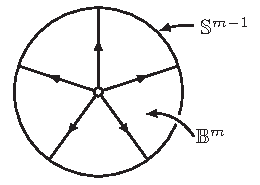
\includegraphics[width=.36\textwidth]{figures/4-8-1.pdf}\\图 4.8.1\par\medskip
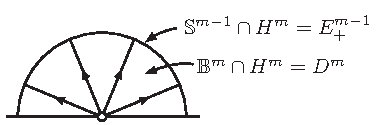
\includegraphics[width=.52\textwidth]{figures/4-8-2.pdf}\\图 4.8.2
\end{center}
从穿孔球到球面的径向形变收缩，限制为 $D^m\setminus\{0\}$ 到 $S^{m-1}\cap\mathbb H^m=E^{m-1}_+$ 的形变收缩。半球体 $D^m$ 为凸集，故无环；半球面 $E^{m-1}_+$ 同胚于 $B^{m-1}$，也无环。由长正合列，二者的相对同调为零，因而得到边界点处的结论。

\entry{定义}{4.8.5}若非空 Hausdorff 空间 $X$ 的每一点都有邻域同胚于 $\R^m$ 的开子集，则称它为\textbf{$m$ 维流形}（$m$-manifold）。若每一点都有邻域同胚于 $\mathbb H^m$ 的开子集，则称它为\textbf{带边界的 $m$ 维流形}（$m$-manifold with boundary）。

每个 $m$ 维流形自动是带边界的流形：若一点的邻域同胚于欧氏开集，可缩小为同胚于开球的邻域，再将此开球同胚地映到以 $(0,\ldots,0,1)$ 为中心的单位开球，它是半空间的开子集。

流形的定义常另外要求有可数基，或至少可度量化。本书不作这两项假设。流形及带边界流形是最熟悉、最重要的几何对象之一，也是微分几何和微分拓扑的主要研究对象。

\sourcepage{230}
若 $h:U\to V$ 将 $X$ 的开集同胚地映到 $\mathbb H^m$ 的开集，则称 $h$ 为 $X$ 上的\textbf{坐标片}（coordinate patch）。一点可能被映入开上半空间，也可能被映到边缘 $\R^{m-1}\times\{0\}$。局部同调区分这两种情况：前者的 $H_m(X,X\setminus\{x\})$ 为无限循环群，后者为零。这引出以下定义。

\entry{定义}{4.8.6}若带边界流形 $X$ 的点 $x$ 在一个坐标片下映入 $\Bd\mathbb H^m$，则在每个坐标片下都如此。称这样的点为 $X$ 的\textbf{边界点}，全体边界点组成的集合称为 $X$ 的\textbf{边界}，记作 $\Bd X$。称 $X\setminus\Bd X$ 为\textbf{内部}，记作 $\Int X$。

定义并不要求边界非空。若边界为空，$X$ 就是通常的 $m$ 维流形。但内部不能空：任一坐标片的像是半空间中的非空开集，必含开上半空间的点，相应的原像就是内部点。半空间 $\mathbb H^m$ 本身是带边界流形，其边界恰是 $\R^{m-1}\times\{0\}$；$\R^m$ 本身也是 $m$ 维流形。

\entry{定义}{4.8.7}由例 4.8.4，$m$ 由空间 $X$ 唯一决定：它是使 $H_m(X,X\setminus\{x\})$ 对至少一个 $x$ 非零的唯一整数。称 $m$ 为带边界流形 $X$ 的\textbf{维数}。

\entry{例}{4.8.8}单位球 $B^n$ 是带边界的 $n$ 维流形，且 $\Bd B^n=S^{n-1}$。若 $p\in B^n\setminus S^{n-1}$，开单位球直接给出坐标片。若 $p\in S^{n-1}$，至少一个坐标非零。不妨设 $p_n<0$。取 $U=\{x\in B^n:x_n<0\}$，定义
\[
h(x)=(x_1,\ldots,x_{n-1},x_n+f(x)),\qquad
f(x)=\sqrt{1-x_1^2-\cdots-x_{n-1}^2}.
\]
可验证 $h$ 将 $U$ 同胚地映到 $V=\{y\in\mathbb H^n:\|y\|<1\}$，且把 $p$ 映到半空间边界，见图 4.8.3。

\sourcepage{231}
\begin{center}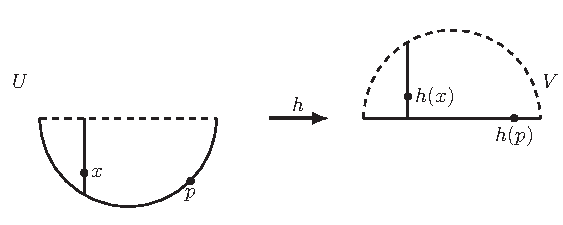
\includegraphics[width=.8\textwidth]{figures/4-8-3.pdf}\\图 4.8.3\end{center}
\entry{例}{4.8.9}任意 $n$ 维单形 $\sigma$ 同胚于 $B^n$，故为带边界的 $n$ 维流形。这个同胚把所有真面的并 $Y$ 映到 $S^{n-1}$。因此，原先记作 $\Bd\sigma$ 的 $Y$，恰为流形意义的边界；原先记作 $\Int\sigma$ 的 $\sigma\setminus Y$，恰为流形意义的内部。

这里有术语重叠，需要澄清。一般拓扑中，若 $A\subset X$，$A$ 的内部是包含于 $A$ 的所有 $X$ 中开集之并；边界是 $\overline A\cap\overline{X\setminus A}$。特别地，当 $A$ 开时，$\Bd A=\overline A\setminus A$。此前本书已用过这些概念，如引理 1.2.7 的 $\Bd U$，以及切除公理中的 $\Int A$。

流形的边界和内部是不同的概念。同一术语有两种用法颇不方便。有些作者用 $\partial X$ 表示流形边界，但这又不易与单纯链 $\partial\sigma$ 区分。我们只好依上下文辨明。对于 $B^n\subset\R^n$，这两种边界碰巧相同；$\mathbb H^n\subset\R^n$ 也是如此，但应把它们视为特殊情况。

下面证明一个关于流形三角剖分的结果。

\sourcepage{232}
\entry{引理}{4.8.10}若 $s$ 是复形 $K$ 的单形，$x,y\in\Int s$，则 $|K|$ 在 $x,y$ 处的局部同调群同构。

\textbf{证明：}只需证明 $x=\widehat s$ 为重心的情形。在第一次重心重分 $\operatorname{sd}K$ 的构造中，将 $s$ 的重心替换为 $y$，即从 $y$ 而非 $\widehat s$ 对 $\Bd s$ 的重分取星，得到重分 $K'$。存在从 $\operatorname{sd}K$ 到 $K'$ 的线性同构，将 $\widehat s$ 映到 $y$，其余顶点不动。因此空间偶 $(|K|,|K|\setminus\{\widehat s\})$ 与 $(|K|,|K|\setminus\{y\})$ 同胚。\hfill$\square$

回忆同胚 $h:|K|\to M$ 称为 $M$ 的\textbf{三角剖分}。任意流形能否三角剖分的问题，经历了约一个世纪的研究。初始猜想可追溯到 Poincar\'e 1899 年的论文，\footnote{Poincar\'e 的拓扑学著作译文见 [Poi10]；第 105--109 页与三角剖分有关。那里的论证尚不满足现代的严格性标准。}Kneser 的 1924 年论文 [Kne25] 为相关问题引入了“Hauptvermutung”这一名称。简言之，所有二维、三维拓扑流形均可三角剖分，而四维及更高维存在不可三角剖分的拓扑流形。较详细而简短的讨论见 [Man14]。

\entry{定理}{4.8.11}若 $M$ 为带边界的 $m$ 维流形，$h:|K|\to M$ 为同胚，则 $h^{-1}(\Bd M)$ 是 $K$ 的某个子复形的多面体。

\textbf{证明：}若开单形 $\Int s$ 与该集合相交，由上一个引理，它完全包含于该集合。因该集合闭，也包含 $s$。\hfill$\square$

最后应用局部同调证明：有限维单纯复形 $K$ 的维数是 $|K|$ 的拓扑不变量。第 2.4、2.7 节习题曾用覆盖维数给出另一种证明的轮廓。先证两个引理。

\entry{引理}{4.8.12}若 $v*L$ 是复形 $L$ 上的锥，则 $|L|$ 是 $|v*L|\setminus\{v\}$ 的形变收缩核。

\textbf{证明：}考虑商映射 $\pi:|L|\times I\to|v*L|$，$\pi(x,t)=(1-t)x+tv$（推论 2.8.8）。集合 $|L|\times[0,1)$ 开且饱和，因此其限制是到 $|v*L|\setminus\{v\}$ 的商映射。它一一对应，故为同胚。再由 $|L|\times\{0\}$ 是 $|L|\times[0,1)$ 的形变收缩核，即得结论。\hfill$\square$

\sourcepage{233}
回忆顶点 $v$ 的星 $\operatorname{St}v$ 是所有含 $v$ 为顶点的单形的内部之并，其链环为 $\operatorname{Lk}v=\overline{\operatorname{St}v}\setminus\operatorname{St}v$。

\entry{引理}{4.8.13}若 $v$ 是 $K$ 的顶点，则
\[
H_i(|K|,|K|\setminus\{v\})\cong H_i(\overline{\operatorname{St}v},\operatorname{Lk}v).
\]
\textbf{证明：}闭星包含 $v$ 的邻域，故引理 4.8.2 给出到 $H_i(\overline{\operatorname{St}v},\overline{\operatorname{St}v}\setminus\{v\})$ 的同构。令 $L$ 为多面体等于 $\operatorname{Lk}v$ 的子复形。由引理 1.9.4，闭星是锥 $v*L$ 的多面体，见图 4.8.4。由上一个引理，链环是穿孔闭星的形变收缩核，即得结论。\hfill$\square$
\begin{center}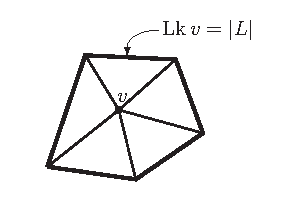
\includegraphics[width=.45\textwidth]{figures/4-8-4.pdf}\\图 4.8.4\end{center}

\entry{定理}{4.8.14}设 $K$ 为 $n$ 维复形，$X=|K|$。当 $p>n$ 时，每个局部同调群 $H_p(X,X\setminus\{x\})$ 都为零；而 $p=n$ 时，至少有一点 $x$ 使该群非零。

\textbf{证明：}取 $K$ 的一个 $n$ 维单形 $\sigma$。它不是其他单形的真面，故 $\Int\sigma$ 在 $|K|$ 中开：其补集为除 $\sigma$ 外所有单形之并。取 $x=\widehat\sigma$，引理 4.8.2 给出
\[
H_n(X,X\setminus\{x\})\cong H_n(\sigma,\sigma\setminus\{\widehat\sigma\})\cong H_n(B^n,B^n\setminus\{0\}),
\]
由例 4.8.3，后者为无限循环群。

对任意 $x$，由引理 4.8.10，只需考虑它是某个单形重心的情形。于是 $x$ 是 $L=\operatorname{sd}K$ 的顶点，由上一个引理，
\[
H_p(X,X\setminus\{x\})\cong H_p(\overline{\operatorname{St}(x,L)},\operatorname{Lk}(x,L)).
\]
\sourcepage{234}
\translatornote{原书此式左端下标误印为 $n$；应与右端同为 $p$。}右端可按奇异同调或单纯同调计算。闭星是维数至多为 $n$ 的复形的多面体，所以 $p>n$ 时，其相对单纯链群为零，同调为零，因而奇异同调也为零。\hfill$\square$

下面三个定义将在习题中使用。

\entry{定义}{4.8.15}若对任意 $x,y\in X$，都有 $X$ 到自身的同胚将 $x$ 映到 $y$，称 $X$ 为\textbf{齐性空间}（homogeneous space）。

\entry{定义}{4.8.16}若空间或复形的同调群与 $S^n$〔相应地，与 $B^n$〕相同，则称为\textbf{$n$ 维同调球面}（homology sphere）〔相应地，\textbf{同调球}（homology ball）〕。

\entry{定义}{4.8.17}\textbf{实心环面}（solid torus）是同胚于 $S^1\times B^2$ 的空间。它是带边界的三维流形，边界同胚于环面。

\subsection*{习题}
\begin{enumerate}
\item 验证例 4.8.8 的细节。
\item 证明：若 $M,N$ 分别为 $m,n$ 维带边界流形，则 $M\times N$ 为 $m+n$ 维带边界流形，且
\[
\Bd(M\times N)=(M\times\Bd N)\cup(\Bd M\times N).
\]
\item 证明连通流形是齐性的。〔提示：若有自身同胚把 $x$ 映到 $y$，定义 $x\sim y$。证明这是等价关系，且每个等价类开。〕
\item 设 $h:|K|\to M$ 是带边界的 $m$ 维流形的三角剖分。
\begin{enumerate}[label=(\alph*)]
\item 证明：顶点 $v$ 的链环在 $h(v)\in\Int M$ 时是 $(m-1)$ 维同调球面，在 $h(v)\in\Bd M$ 时是同调球。
\item 证明 $K$ 的每个单形或为 $m$ 维，或是某个 $m$ 维单形的面。
\item 证明：若 $(m-1)$ 维单形 $s\subset h^{-1}(\Bd M)$，则它恰是一个 $m$ 维单形的面；否则恰是两个 $m$ 维单形的面。
\end{enumerate}
\item 利用 $S^3$ 同胚于 $\Bd(B^2\times B^2)$，把 $S^3$ 写成两个实心环面 $T_1,T_2$ 之并，使其交为共同边界。计算相应 Mayer--Vietoris 序列。
\item 设 $C$ 为实数轴中的 Cantor 三分集（定义 2.3.13）。$C$ 的维数是多少？
\item 给出 $\R^3$ 中一个一维集合的例子，再给出一个二维集合的例子。
\end{enumerate}
